\documentclass{article}

\usepackage[english]{babel}
\usepackage[style=abnt,backend=biber,citecounter=true,backrefstyle=three]{biblatex}
\usepackage[letterpaper,top=2cm,bottom=2cm,left=3cm,right=3cm,marginparwidth=1.75cm]{geometry}
\usepackage{float}

\usepackage{amsmath}
\usepackage{graphicx}
\usepackage[colorlinks=true, allcolors=blue]{hyperref}

\title{Trabalho MPI: Análise de Desempenho de Estratégias de Comunicação}
\author{Henrique Utzig e Pedro Afonso Klein}

\begin{document}
\maketitle

\section{Introdução}
\

A multiplicação de matrizes é uma operação muito comum em diversas áreas da ciência e engenharia, sendo bastante utilizada como um benchmark para testar o desempenho de sistemas paralelos. O objetivo deste trabalho é comparar o desempenho de diferentes estratégias de comunicação MPI para um algoritmo que realiza essa multiplicação.

Nossa análise busca entender como cada método de comunicação afeta a eficiência geral do programa. Para isso, medimos métricas como o tempo total de execução, o tempo gasto apenas na comunicação e o tempo gasto no cálculo, variando a carga de trabalho. Partindo de um código base fornecido, avaliamos as seguintes abordagens:

\begin{itemize}
    \item Comunicação ponto-a-ponto bloqueante;
    \item Comunicação ponto-a-ponto não bloqueante;
    \item Comunicação com operações coletivas.
\end{itemize}

Neste relatório, vamos detalhar como cada estratégia foi implementada, como os testes foram feitos e, por fim, apresentar e analisar os resultados que obtivemos.

\section{Comunicação Entre Processos}
\

Para começar, recebemos três algoritmos base para a multiplicação de matrizes paralela. Cada um usava um tipo de comunicação diferente: ponto-a-ponto bloqueante, não bloqueante e coletiva. Nós refatoramos e melhoramos esses códigos para poder analisar o desempenho deles.

Em todas as versões, a lógica de distribuição dos dados é parecida: o processo de \texttt{rank 0} cria as matrizes A, B e C. Ele divide a matriz A em faixas de linhas e envia uma para cada um dos outros processos. A grande diferença entre os métodos está em \textbf{como} ele envia essas partes de A e depois recebe os resultados de C. Já a matriz B é enviada inteira para todo mundo usando um broadcast (\texttt{MPI\_Bcast} nas versões síncrona e coletiva, e \texttt{MPI\_Ibcast} na assíncrona).

\subsection{Comunicação Bloqueante}
\

Nesta abordagem, a comunicação é síncrona. O processo de \texttt{rank 0} envia as partes da matriz A para os outros processos usando um laço com a chamada \texttt{MPI\_Send}. Essa chamada é "bloqueante", o que significa que o \texttt{rank 0} fica parado, esperando o processo de destino receber a mensagem com \texttt{MPI\_Recv} para só então continuar.

Da mesma forma, no final, cada processo "trabalhador" envia sua parte calculada da matriz C de volta para o \texttt{rank 0}, que fica em um laço com \texttt{MPI\_Recv} para receber tudo. Essa abordagem é simples, mas pode criar um tempo ocioso considerável, já que os processos ficam parados esperando a comunicação terminar.

\subsection{Comunicação Não-Bloqueante}
\

A versão não bloqueante (ou assíncrona) foi pensada para diminuir esse tempo de espera, usando as chamadas \texttt{MPI\_Isend} e \texttt{MPI\_Irecv}. O \texttt{rank 0} usa \texttt{MPI\_Isend} para começar a enviar os dados e os trabalhadores usam \texttt{MPI\_Irecv} para se preparar para receber. Essas chamadas retornam imediatamente, permitindo que o programa continue executando outras tarefas.

No entanto, na implementação original que recebemos, logo depois da chamada \texttt{MPI\_Irecv}, o código já usava um \texttt{MPI\_Wait}. Essa chamada bloqueia o processo até que a comunicação termine. Na prática, isso acaba fazendo com que a comunicação "não bloqueante" se comporte como uma bloqueante, perdendo a principal vantagem do método: a chance de fazer cálculos enquanto os dados são transferidos. O mesmo padrão acontece na hora de coletar os resultados e também para distribuir a matriz B com \texttt{MPI\_Ibcast}, que é seguido de um \texttt{MPI\_Wait}.

\subsection{Comunicação Coletiva}
\

Esta estratégia usa operações de comunicação coletiva do MPI, que são feitas sob medida para situações onde todos os processos precisam se comunicar. Para distribuir a matriz A, usamos a função \texttt{MPI\_Scatter}. Com ela, o processo raiz (\texttt{rank 0}) divide a matriz A e distribui uma parte para cada processo.

Depois do cálculo, a função \texttt{MPI\_Gather} faz o inverso: cada processo envia seu resultado para o processo raiz, que junta tudo na matriz C final. Essas operações são bloqueantes, mas geralmente são muito eficientes, pois a própria biblioteca MPI usa algoritmos otimizados para a rede do sistema.

\subsubsection{Melhorias no código base}
\

Como a versão não bloqueante original acabava sendo síncrona por causa do uso imediato do \texttt{MPI\_Wait}, criamos uma nova versão que chamamos de \texttt{async\_new}. Nela, os processos trabalhadores postam os recebimentos da matriz A (\texttt{MPI\_Irecv}) e da matriz B (\texttt{MPI\_Ibcast}) e depois usam uma única chamada \texttt{MPI\_Waitall} para esperar que as duas transferências terminem. Isso permite que os dados de A e B cheguem ao mesmo tempo, o que pode diminuir o tempo de comunicação. Mesmo assim, vale notar que o cálculo só começa depois que todos os dados chegam.

Além disso, o código base foi bastante refatorado para facilitar os testes. Separamos cada estratégia em seu próprio arquivo e criamos um \texttt{main.c} para controlar a execução. Adicionamos também um sistema para escolher o tipo de comunicação e o tamanho da matriz pela linha de comando, com opções como \texttt{--verbose} e \texttt{--validate}. A flag \texttt{--validate} executa o cálculo de forma sequencial e compara com o resultado paralelo, para garantir que nossos algoritmos estavam corretos.

\section{Metodologia de Testes}
\

Para comparar as estratégias de forma justa e confiável, definimos uma metodologia de testes bem clara. Nesta seção, explicamos como as métricas foram coletadas e como os testes foram executados.

\subsection{Medidas de Tempo}
\

Para medir o desempenho, focamos em três tempos: total, de comunicação e de computação, usando a função \texttt{MPI\_Wtime()}. Em vez de medir o tempo apenas no \texttt{rank 0}, cada processo mediu seus próprios tempos. No final, usamos uma operação \texttt{MPI\_Reduce} com \texttt{MPI\_MAX} para pegar o maior tempo de comunicação e o maior tempo de computação entre todos os processos. Essa abordagem é importante porque o desempenho de um programa paralelo é limitado pelo seu processo mais lento (o gargalo).

\subsection{Testes Iniciais}
\

Fizemos alguns testes exploratórios no cluster "Hype" para entender o comportamento do código, usando matrizes de 512x512 e 8192x8192 com 32 processos.

Ao rodar os testes em vários nós (2, 3 e 4), percebemos um atraso considerável antes mesmo do nosso programa começar a executar. Esse tempo extra provavelmente vem do trabalho que o SLURM e o MPI têm para alocar os recursos, iniciar os processos e configurar a comunicação entre as máquinas. Para problemas pequenos, esse tempo de inicialização pode acabar dominando o tempo total. Tentamos usar a flag "bind-to core" do "mpirun", mas não tivemos sucesso, uma vez que ele tentava vincular cada um dos 32 processos a um core físico, mas os nodos da "Hype" tem apenas 20 cores físicos.

\subsection{Testes em Lote Automatizados}
\

Para rodar os testes de forma automática e organizada, criamos um script em Python (\texttt{batch\_test.py}). A bateria final de testes foi configurada com os seguintes parâmetros:
\begin{itemize}
    \item \textbf{Tamanhos de Matriz:} 512x512, 1024x1024 e 2048x2048.
    
    \item \textbf{Número de Processos:} 32 processos, alocados pelo SLURM (\texttt{--ntasks=32}) em 1, 2, 3 ou 4 nós do cluster "Hype".
    
    \item \textbf{Repetições:} Cada combinação foi executada 3 vezes para podermos calcular a média e o desvio padrão, o que dá mais confiança estatística aos resultados.
    
    \item \textbf{Estratégias:} Todas as quatro versões (\texttt{sync}, \texttt{async}, \texttt{async\_new}, \texttt{collective}) foram testadas sob as mesmas condições.
\end{itemize}

A execução no cluster foi controlada por um script SLURM, e o comando "mpirun" foi configurado com flags específicas para forçar a comunicação a usar a rede TCP/IP padrão, garantindo que os resultados fossem comparáveis:

\begin{verbatim}
mpirun -np 32 -machinefile ... \
  --mca btl ^openib --mca btl_tcp_if_include eno2 \
  --mca mtl ^ofi ...
\end{verbatim}

Essas flags instruem o MPI a ignorar a rede de alta velocidade InfiniBand (\texttt{openib}) e usar a rede Ethernet padrão (\texttt{eno2}). Isso evita variações de desempenho causadas por diferentes hardwares de rede.

\section{Resultados e Análise}
\

Nesta seção, apresentamos e analisamos os resultados dos testes. O foco é no tempo de comunicação e de computação para cada uma das quatro estratégias, variando o tamanho da matriz e o número de nós (de 1 a 4), sempre com 32 processos no total.

\subsection{Tempo de Comunicação de Cada Estratégia}
\

O tempo de comunicação é um ponto chave em aplicações distribuídas, pois é o custo extra que pagamos por dividir o trabalho. As figuras \ref{fig:comm_time_1} a \ref{fig:comm_time_4} mostram o tempo médio de comunicação para cada estratégia, com barras de erro indicando o desvio padrão.

\begin{figure}[H]
    \centering
    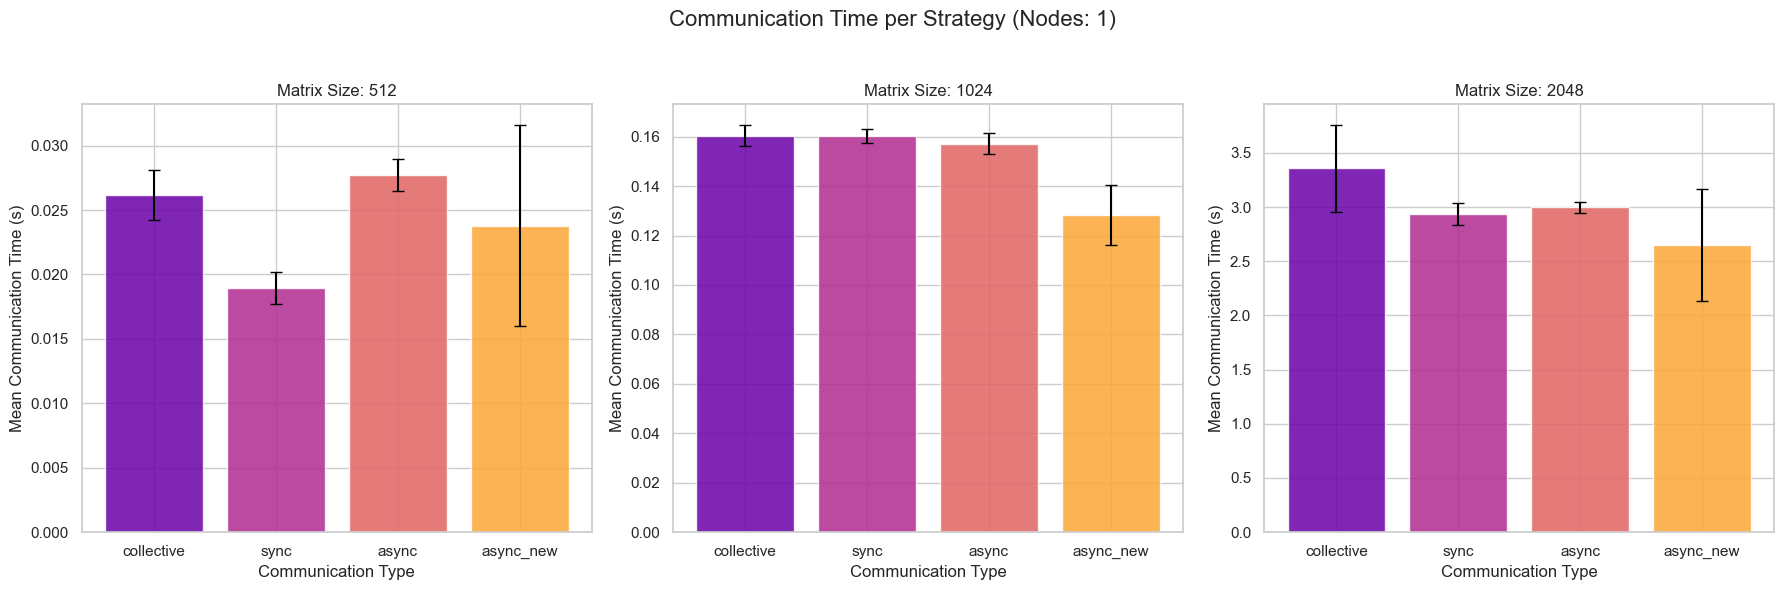
\includegraphics[width=1\linewidth]{images/comm_time_1node.png}
    \caption{Tempo de comunicação por estratégia com 1 nó.}
    \label{fig:comm_time_1}
\end{figure}

\begin{figure}[H]
    \centering
    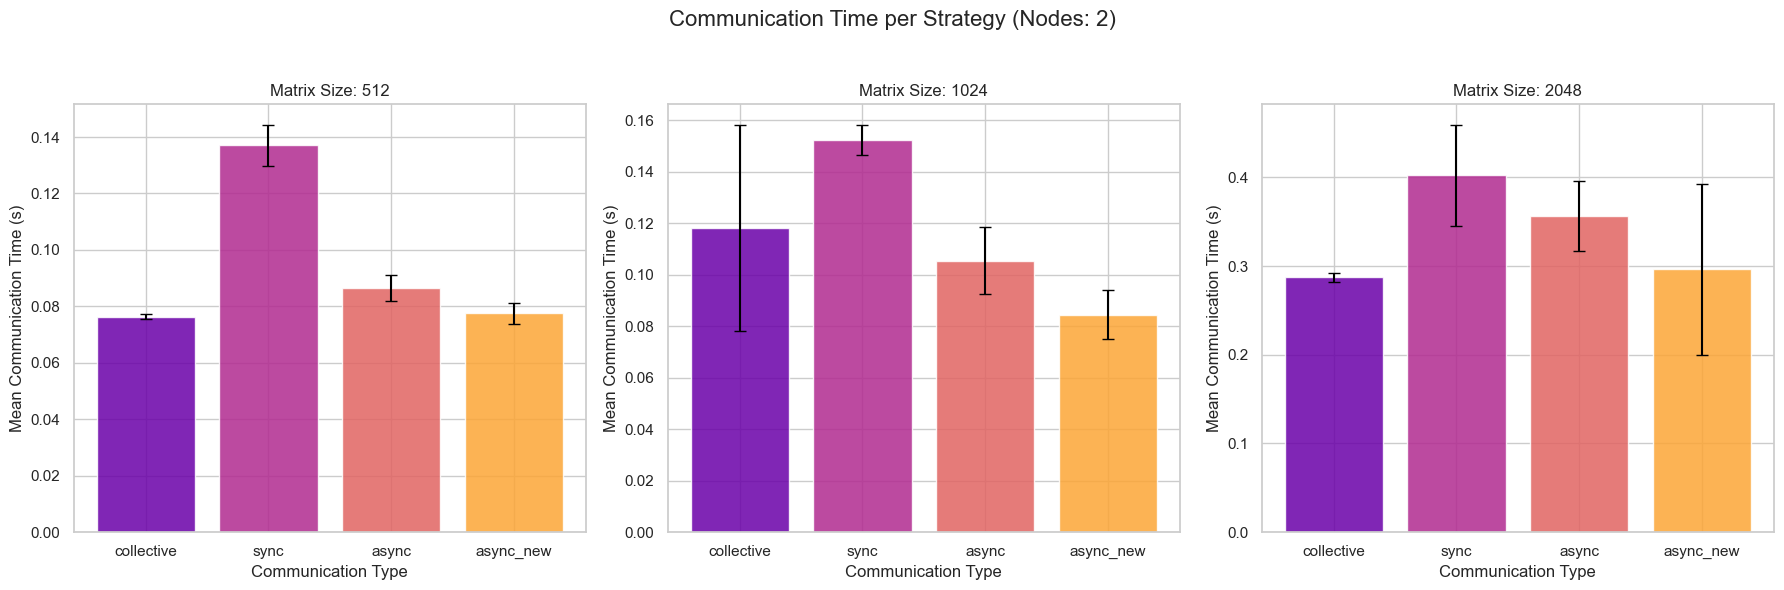
\includegraphics[width=1\linewidth]{images/comm_time_2nodes.png}
    \caption{Tempo de comunicação por estratégia com 2 nós.}
    \label{fig:comm_time_2}
\end{figure}

\begin{figure}[H]
    \centering
    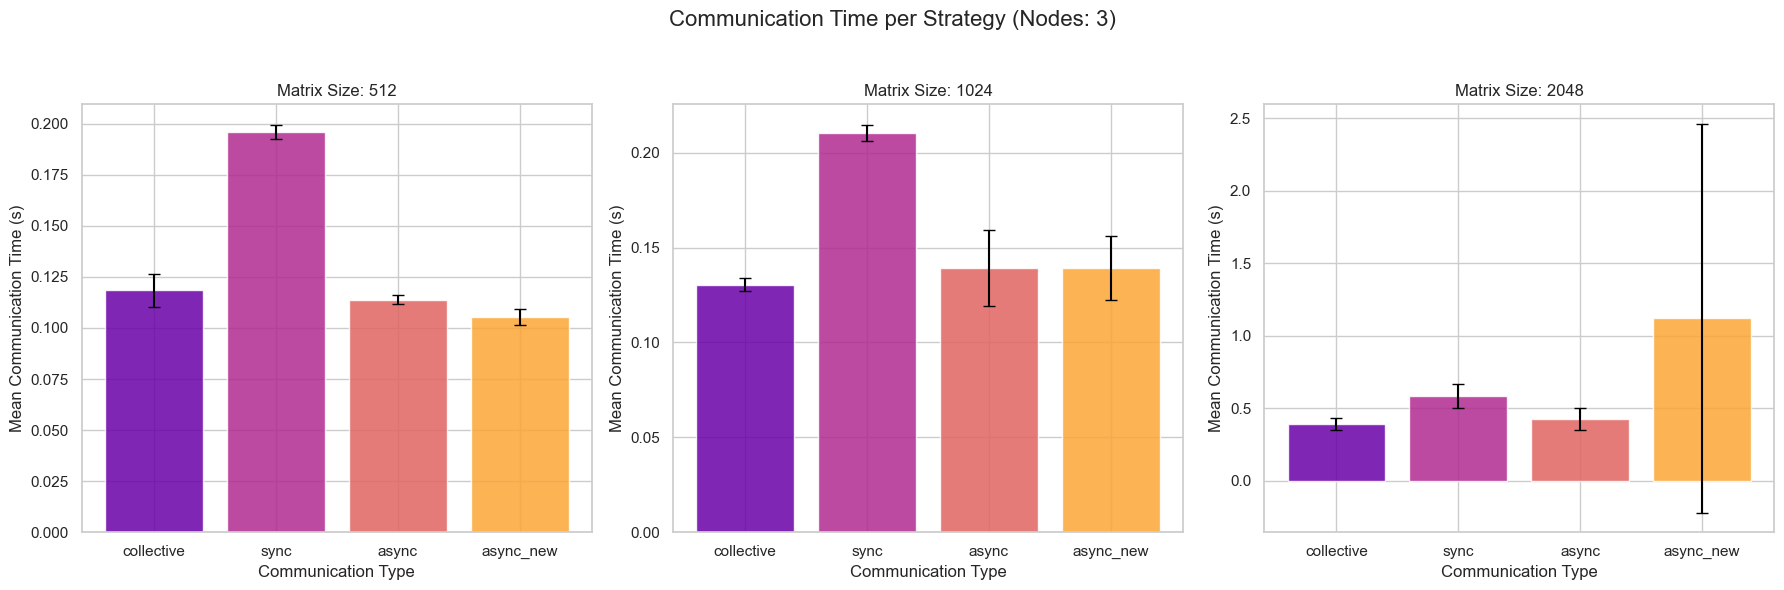
\includegraphics[width=1\linewidth]{images/comm_time_3nodes.png}
    \caption{Tempo de comunicação por estratégia com 3 nós.}
    \label{fig:comm_time_3}
\end{figure}

\begin{figure}[H]
    \centering
    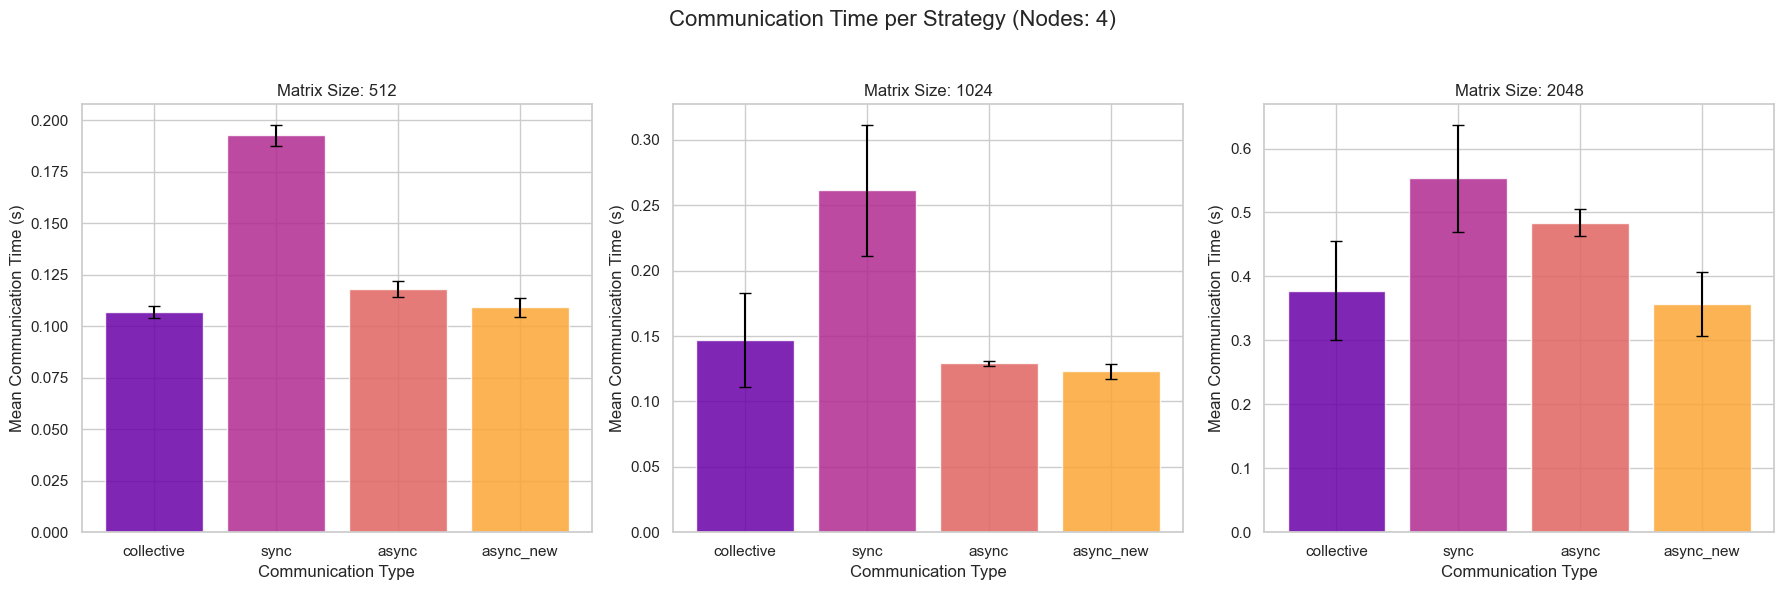
\includegraphics[width=1\linewidth]{images/comm_time_4nodes.png}
    \caption{Tempo de comunicação por estratégia com 4 nós.}
    \label{fig:comm_time_4}
\end{figure}

Olhando os gráficos, percebemos padrões diferentes dependendo do ambiente.

\textbf{Em um único nó (Figura \ref{fig:comm_time_1})}, a comunicação acontece pela memória, então não há o atraso da rede. Curiosamente, para a matriz menor (512x512), a comunicação síncrona (\texttt{sync}) foi a mais rápida. Isso sugere que, com poucos dados, o trabalho extra para configurar as comunicações coletivas e não bloqueantes acaba não compensando. Mas, conforme a matriz aumenta, a estratégia \texttt{async\_new} se torna a mais eficiente, mostrando que ela lida bem com volumes maiores de dados.

\textbf{Em múltiplos nós (Figuras \ref{fig:comm_time_2}, \ref{fig:comm_time_3} e \ref{fig:comm_time_4})}, a história muda completamente. A latência da rede prejudica muito a abordagem bloqueante. A estratégia \texttt{sync} se torna a pior em todos os cenários com mais de um nó, pois os processos ficam muito tempo ociosos, esperando os dados chegarem pela rede.

Por outro lado, as estratégias \texttt{collective} e \texttt{async\_new} se destacam como as mais rápidas.
\begin{itemize}
    \item A abordagem \textbf{\texttt{collective}} se mostrou extremamente robusta e eficiente, principalmente com grandes volumes de dados, o que mostra como os algoritmos da biblioteca MPI são bem otimizados.
    \item A nossa implementação \textbf{\texttt{async\_new}} foi igualmente forte, e em alguns casos até superou a coletiva. Isso sugere que sua arquitetura, que lida com múltiplas transferências ao mesmo tempo, escala muito bem quando o número de nós aumenta.
    \item A versão original \textbf{\texttt{async}} ficou no meio termo. Foi melhor que a \texttt{sync} em múltiplos nós, mas sempre perdeu para a \texttt{collective} e a \texttt{async\_new}, confirmando que seu padrão "Irecv-Wait" não aproveita bem o potencial da comunicação assíncrona.
\end{itemize}

\subsection{Porcentagem de Comunicação e Computação de Cada Estratégia}
\

Para entender melhor onde o tempo é gasto, geramos gráficos que mostram a proporção de tempo de comunicação versus computação. As figuras \ref{fig:comp_time_1} a \ref{fig:comp_time_4} mostram essa divisão.

Uma observação importante sobre estes gráficos: as porcentagens são calculadas com base na soma do tempo máximo de comunicação e do tempo máximo de computação. Como o processo mais lento na comunicação pode não ser o mesmo que o mais lento no cálculo, essa soma não é exatamente igual ao tempo total de execução. Mesmo assim, essa abordagem nos dá uma ótima ideia se a aplicação é limitada pela comunicação ou pelo cálculo.

\begin{figure}[H]
    \centering
    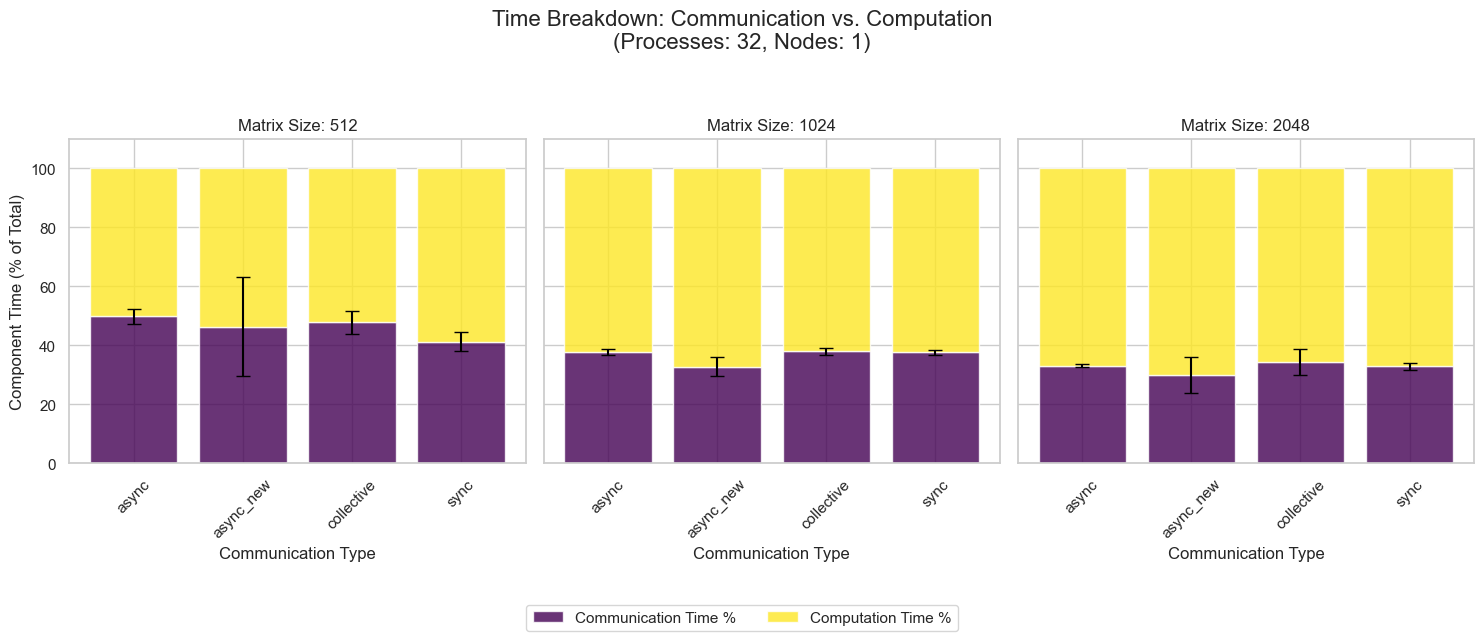
\includegraphics[width=1\linewidth]{images/comp_time_1node.png}
    \caption{Porcentagem de comunicação e computação por estratégia com 1 nó.}
    \label{fig:comp_time_1}
\end{figure}

\begin{figure}[H]
    \centering
    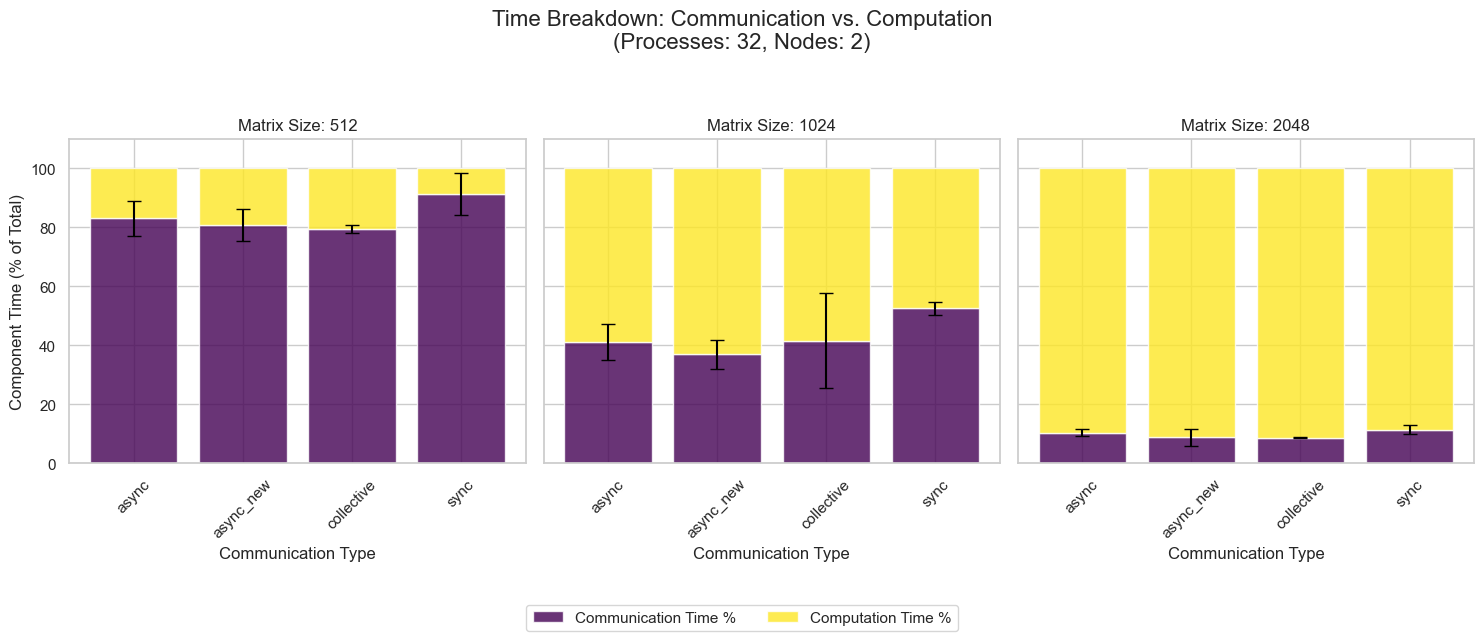
\includegraphics[width=1\linewidth]{images/comp_time_2nodes.png}
    \caption{Porcentagem de comunicação e computação por estratégia com 2 nós.}
    \label{fig:comp_time_2}
\end{figure}

\begin{figure}[H]
    \centering
    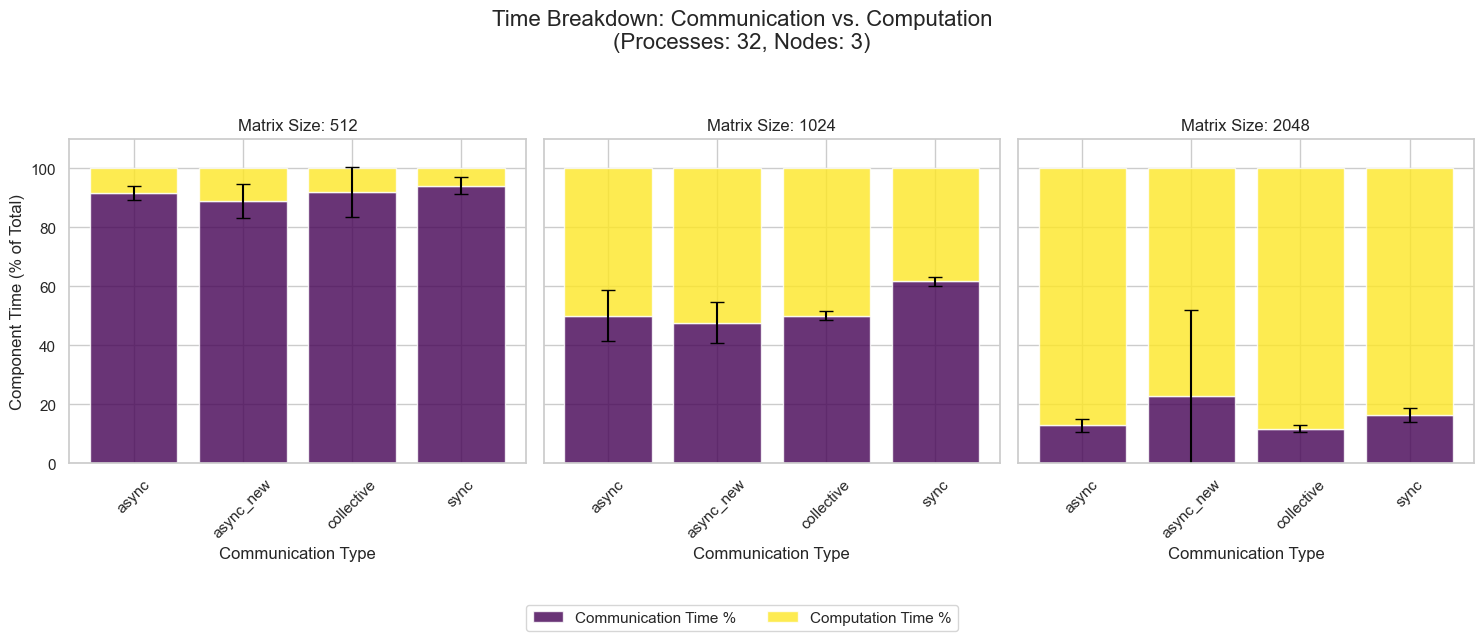
\includegraphics[width=1\linewidth]{images/comp_time_3nodes.png}
    \caption{Porcentagem de comunicação e computação por estratégia com 3 nós.}
    \label{fig:comp_time_3}
\end{figure}

\begin{figure}[H]
    \centering
    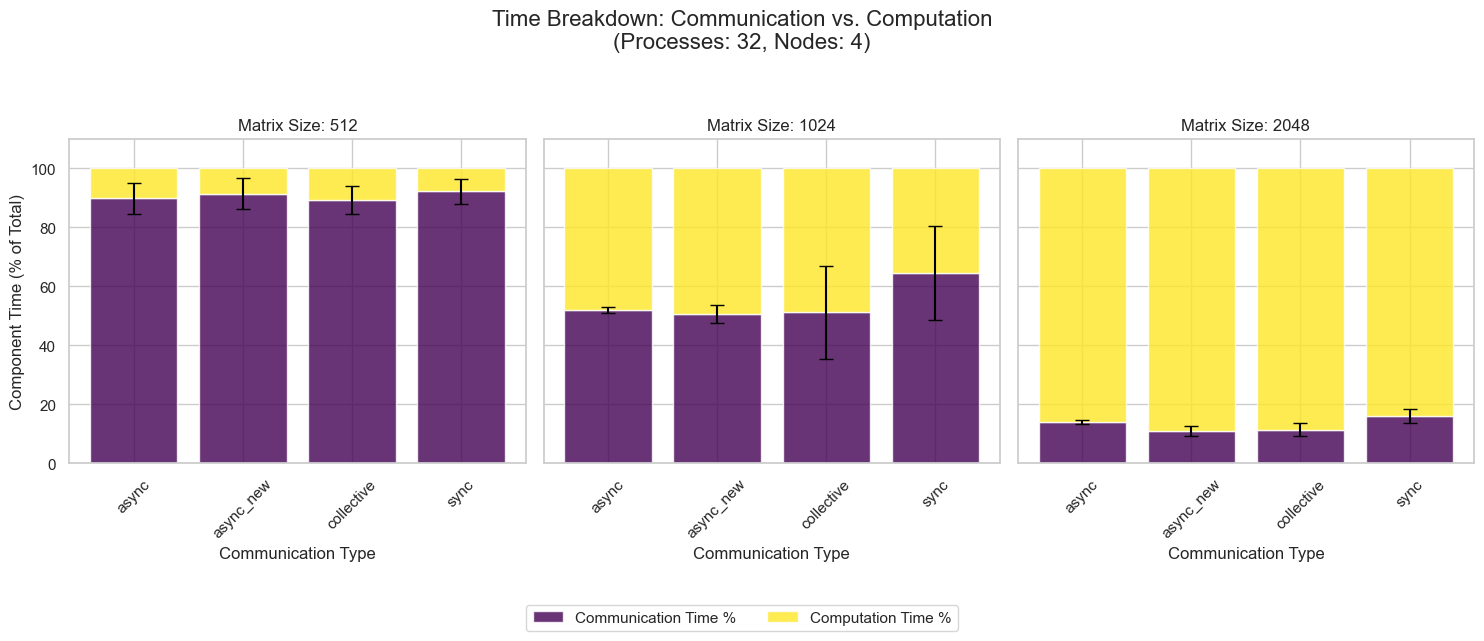
\includegraphics[width=1\linewidth]{images/comp_time_4nodes.png}
    \caption{Porcentagem de comunicação e computação por estratégia com 4 nós.}
    \label{fig:comp_time_4}
\end{figure}

A análise dos gráficos revela duas tendências principais:

1.  \textbf{Impacto do Tamanho da Matriz:} Em todos os cenários, quanto maior a matriz, maior a proporção de tempo gasta em computação (barra amarela). Para a matriz de 512x512, a comunicação domina, mas para a de 2048x2048, o cálculo se torna a atividade principal. Isso é esperado, já que a complexidade do cálculo cresce mais rápido ($O(n^3)$) do que o volume de dados para comunicação ($O(n^2)$).

2.  \textbf{Impacto do Aumento de Nós (Escalabilidade):} Para um mesmo tamanho de matriz, adicionar mais nós tende a aumentar a porcentagem de tempo gasta em comunicação. Isso fica bem claro com a matriz de 512x512: com 4 nós, a comunicação passa de 90\% do tempo. Isso mostra um limite de escalabilidade: o problema fica tão pequeno para cada processo que o custo de se comunicar se torna o gargalo principal. Em contraste, para a matriz de 2048x2048, o cálculo continua dominante mesmo com 4 nós, mostrando que a paralelização é eficiente para problemas grandes.

A estratégia \texttt{sync} sempre mostra a maior porcentagem de tempo de comunicação em múltiplos nós, o que reforça visualmente o quão ineficiente ela é. Já as estratégias \texttt{collective} e \texttt{async\_new} mantêm um equilíbrio melhor, permitindo que os processos passem mais tempo calculando.

\subsection{Diferença no tempo medido vs calculado}
\

Como explicamos na metodologia, medimos o tempo de comunicação e computação pegando o valor máximo entre todos os processos. No entanto, a soma desses máximos (\texttt{max(comm) + max(comp)}) nem sempre bate com o tempo total de execução. Tentamos entender por que essa diferença acontece.

O motivo é algo comum em sistemas paralelos: o processo que mais demora para comunicar não é, necessariamente, o que mais demora para calcular. O tempo total é ditado pelo "caminho crítico", ou seja, pelo último processo a terminar tudo. A diferença entre o tempo total medido e a soma dos máximos, portanto, revela o nível de desbalanceamento de carga e sobreposição de tarefas. As figuras \ref{fig:time_imbalance_1} a \ref{fig:time_imbalance_4} comparam esses valores.

\begin{figure}[H]
    \centering
    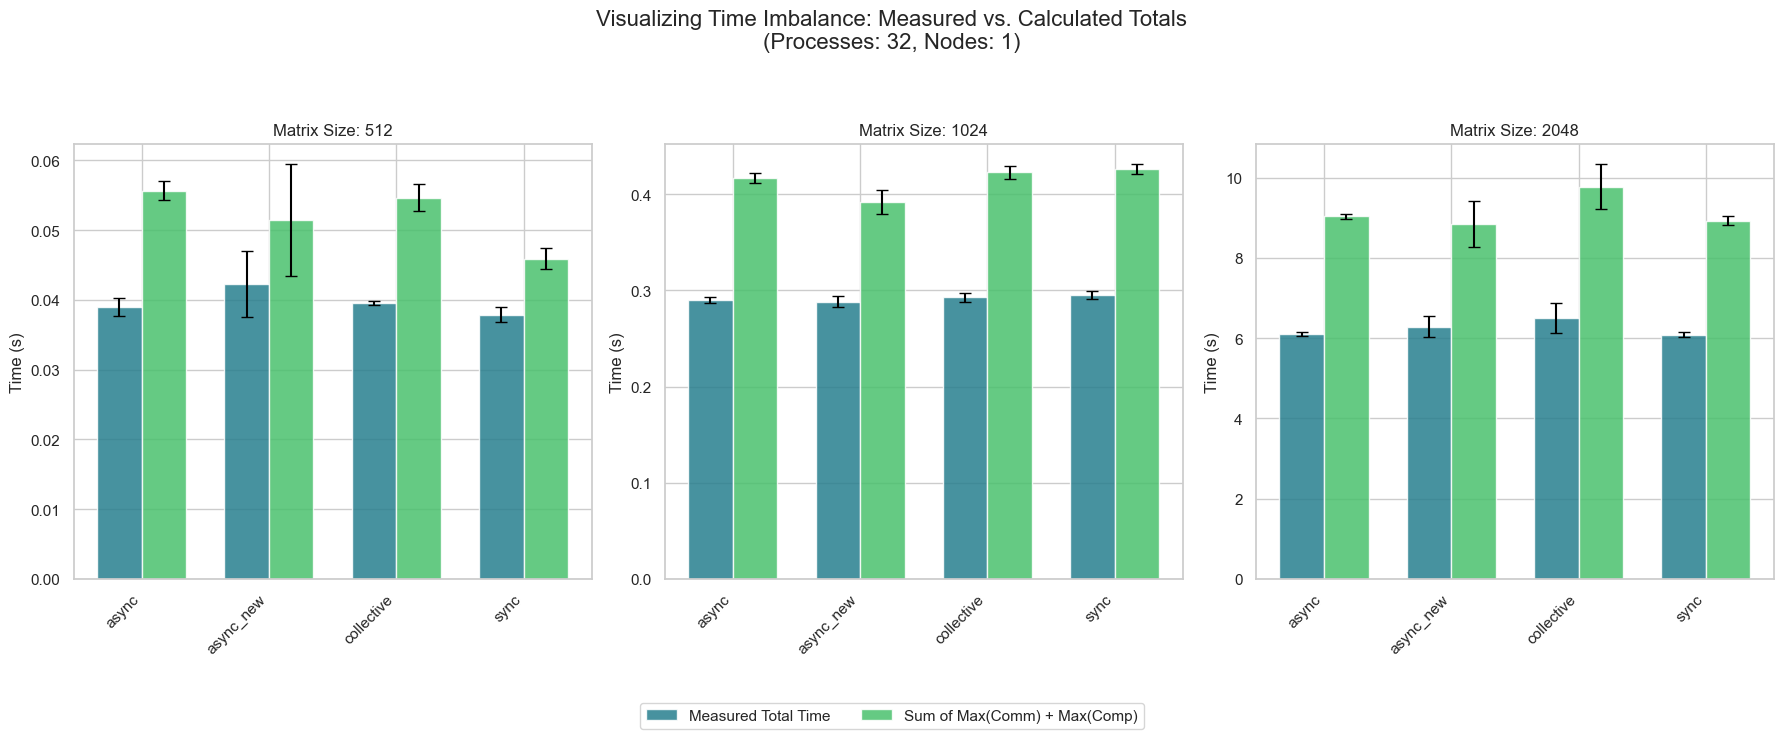
\includegraphics[width=1.0\linewidth]{images/time_imbalance_1node.png}
    \caption{Diferença entre tempo medido e calculado a partir dos tempos máximos para 1 nó.}
    \label{fig:time_imbalance_1}
\end{figure}

\begin{figure}[H]
    \centering
    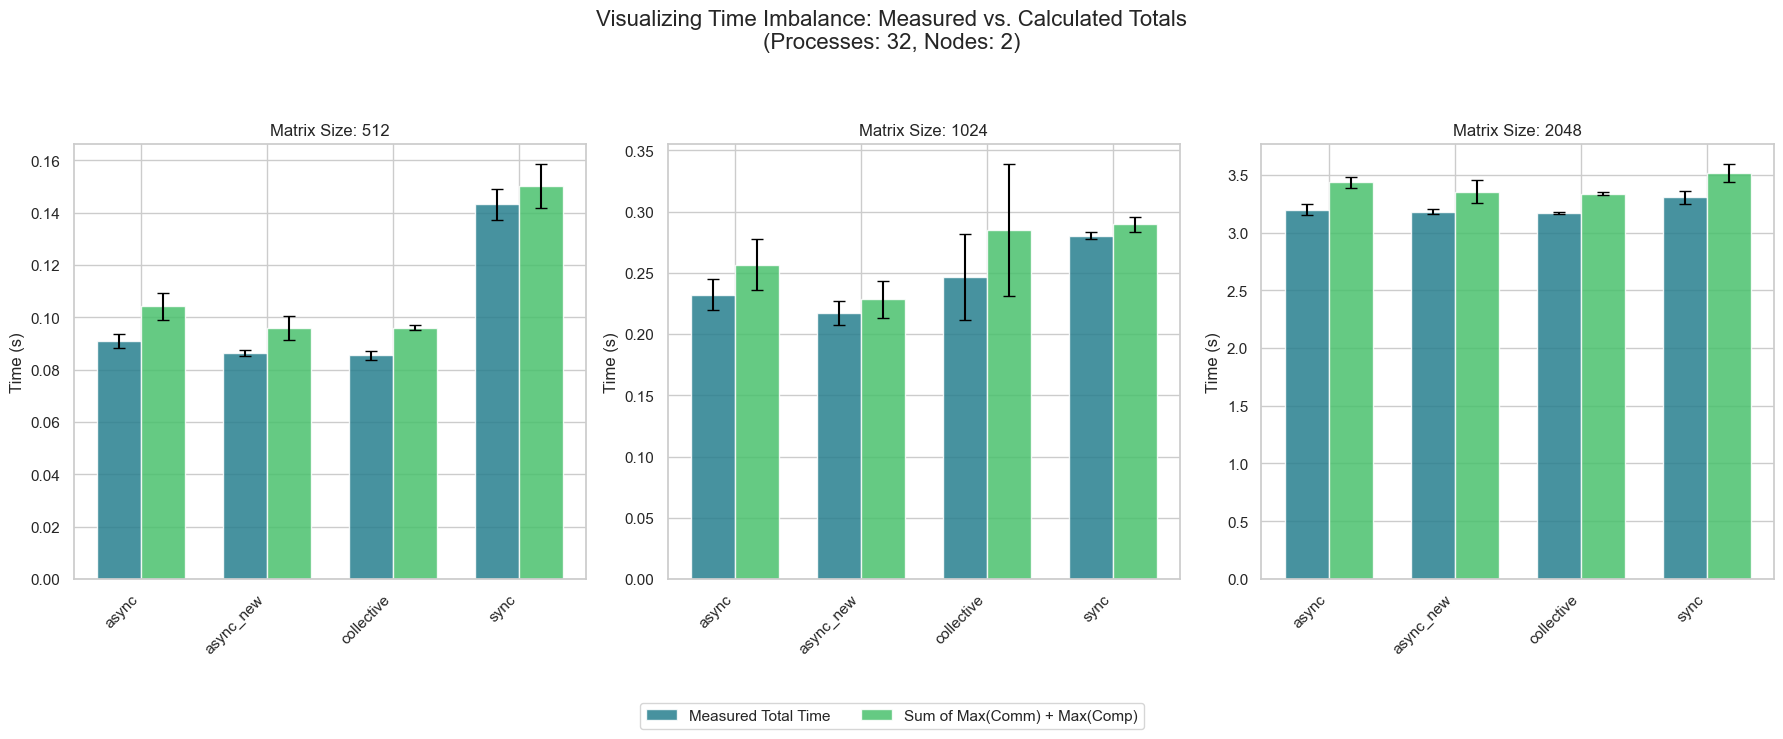
\includegraphics[width=1.0\linewidth]{images/time_imbalance_2nodes.png}
    \caption{Diferença entre tempo medido e calculado a partir dos tempos máximos para 2 nós.}
    \label{fig:time_imbalance_2}
\end{figure}

\begin{figure}[H]
    \centering
    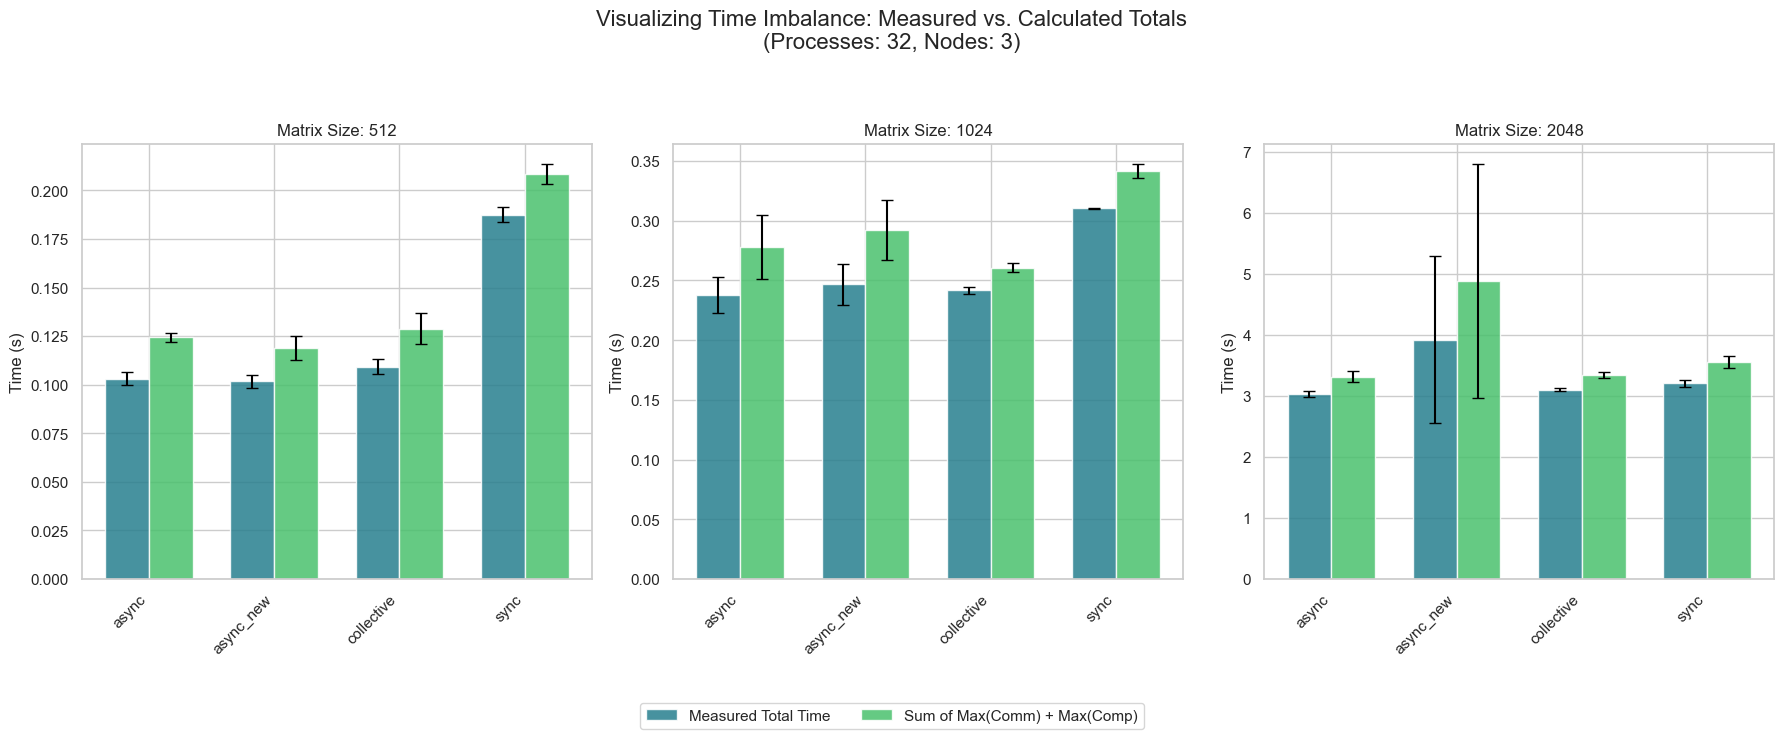
\includegraphics[width=1.0\linewidth]{images/time_imbalance_3nodes.png}
    \caption{Diferença entre tempo medido e calculado a partir dos tempos máximos para 3 nós.}
    \label{fig:time_imbalance_3}
\end{figure}

\begin{figure}[H]
    \centering
    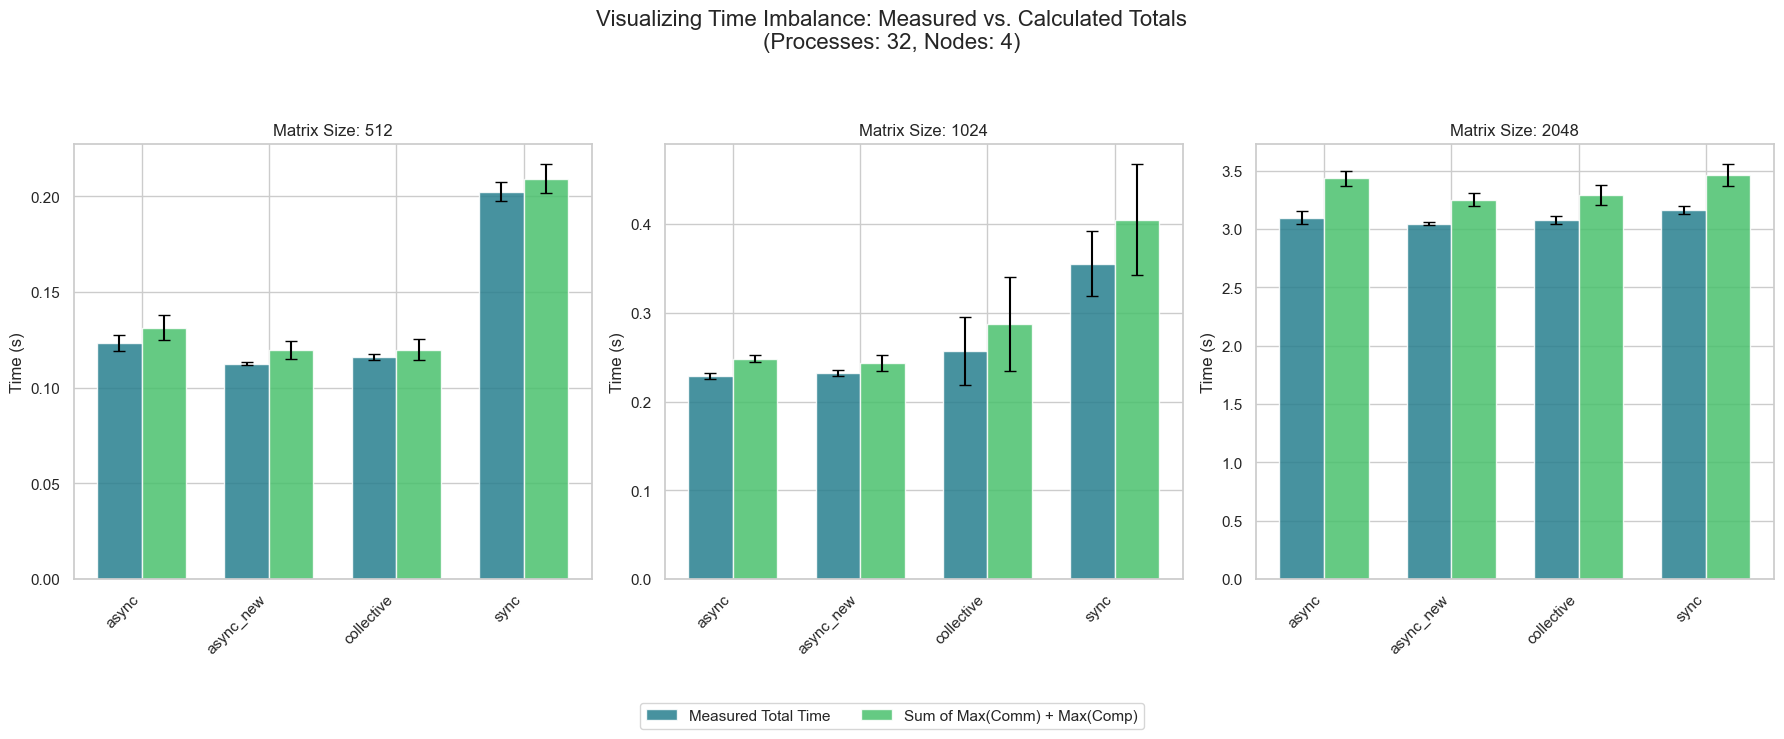
\includegraphics[width=1.0\linewidth]{images/time_imbalance_4nodes.png}
    \caption{Diferença entre tempo medido e calculado a partir dos tempos máximos para 4 nós.}
    \label{fig:time_imbalance_4}
\end{figure}

A análise mostra uma mudança clara quando saímos de um nó para múltiplos nós.

\textbf{Em um único nó (Figura \ref{fig:time_imbalance_1})}, a diferença entre o tempo calculado (soma dos máximos) e o tempo total medido é grande. O tempo calculado superestima o tempo real. Isso acontece porque, dentro de uma máquina, o sistema operacional consegue ser esperto: enquanto um processo está bloqueado esperando dados (comunicação), outro pode estar usando a CPU (computação), gerando uma sobreposição de tarefas que nossa soma simples não captura.

\textbf{Em múltiplos nós (Figuras \ref{fig:time_imbalance_2}, \ref{fig:time_imbalance_3} e \ref{fig:time_imbalance_4})}, a situação se inverte. A diferença entre os tempos diminui muito, e a soma dos máximos se torna uma aproximação bem melhor do tempo real. A latência da rede força uma execução mais "em fila": os processos tendem a receber dados e *depois* calcular, o que reduz a sobreposição.

Essa análise valida nossa metodologia de medição. Ela mostra que, embora \texttt{max(comm)} e \texttt{max(comp)} sejam ótimos para identificar gargalos, o desempenho geral é mais complexo.

\subsection{Impacto da comunicação no tempo total}
\

Esta análise visualiza o impacto absoluto do tempo de comunicação no tempo total. Os gráficos a seguir (Figuras \ref{fig:impact_1node} a \ref{fig:impact_4nodes}) mostram o tempo total de execução na altura da barra, enquanto a área listrada no topo representa quanto desse tempo foi gasto no gargalo de comunicação (\texttt{max(comm)}).

Isso é fundamental, pois conecta a eficiência de uma parte do processo (a comunicação) com o objetivo final: reduzir o tempo total de execução.

\begin{figure}[H]
    \centering
    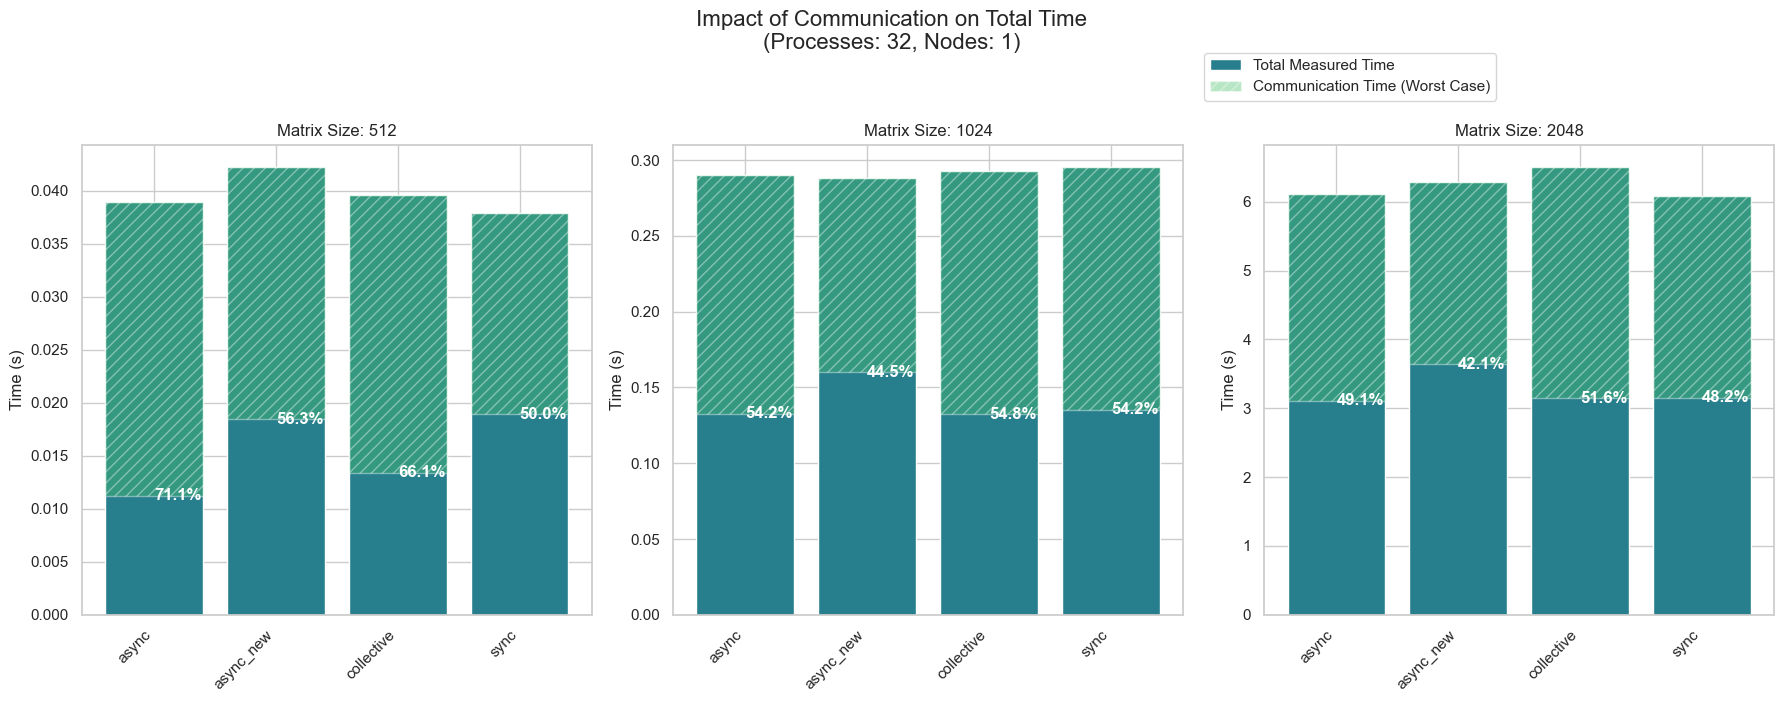
\includegraphics[width=1\linewidth]{images/comm_impact_1node.png}
    \caption{Impacto da comunicação no tempo total para 1 nó.}
    \label{fig:impact_1node}
\end{figure}

\begin{figure}[H]
    \centering
    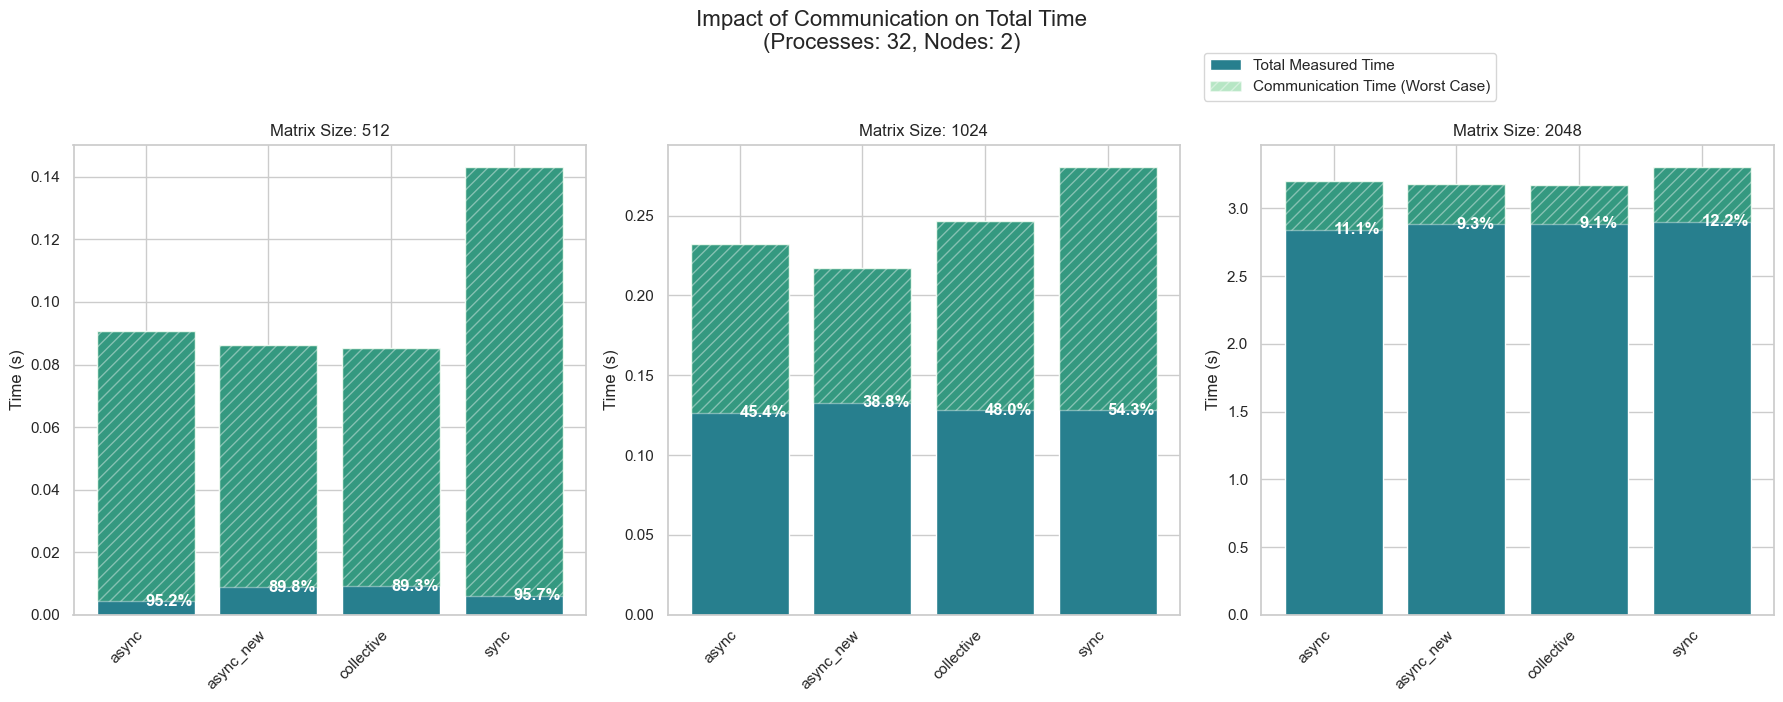
\includegraphics[width=1\linewidth]{images/comm_impact_2nodes.png}
    \caption{Impacto da comunicação no tempo total para 2 nós.}
    \label{fig:impact_2nodes}
\end{figure}

\begin{figure}[H]
    \centering
    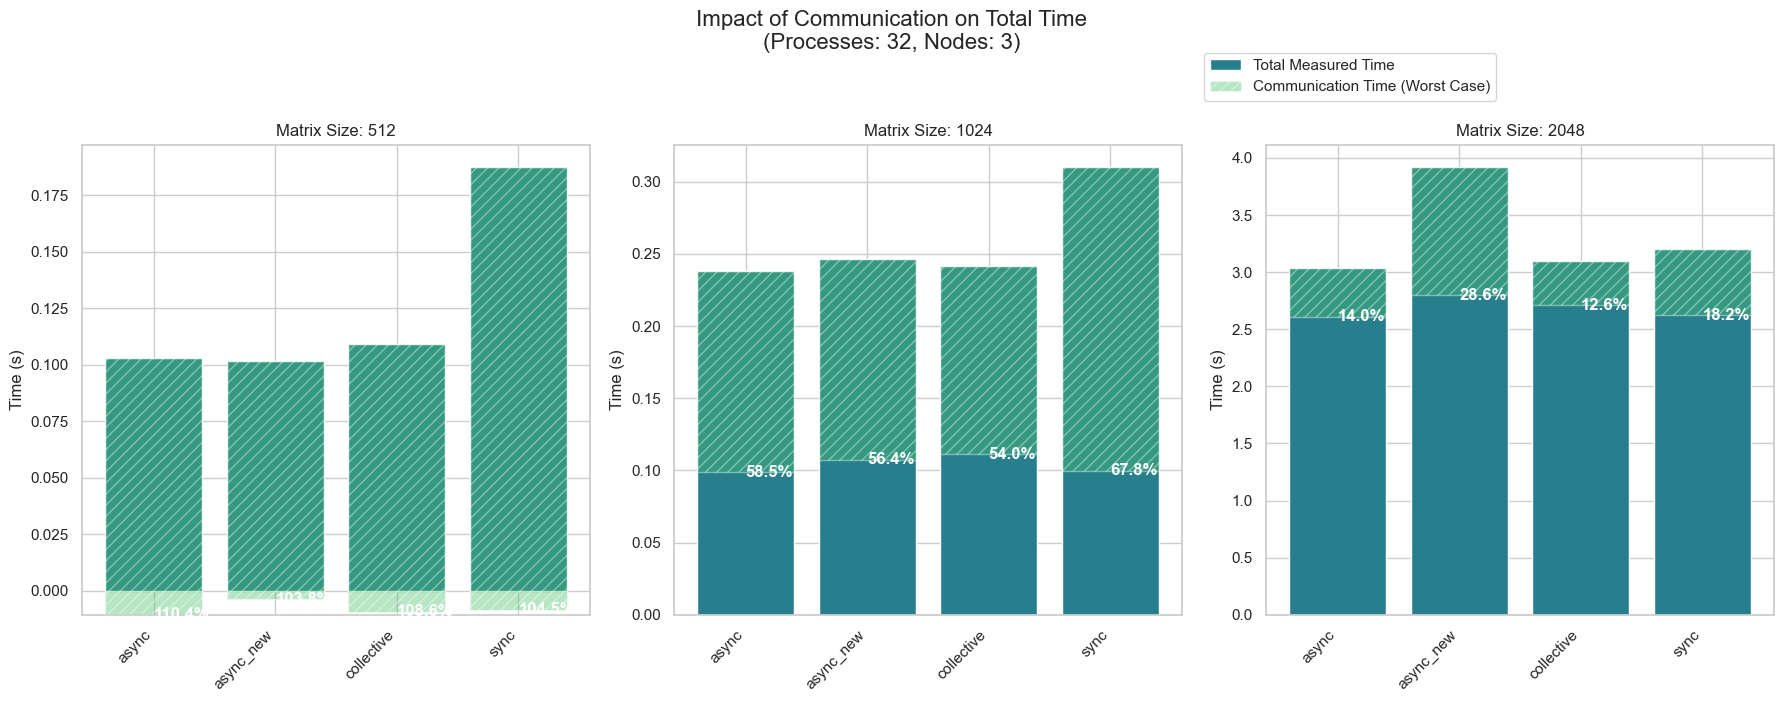
\includegraphics[width=1\linewidth]{images/comm_impact_3nodes.png}
    \caption{Impacto da comunicação no tempo total para 3 nós.}
    \label{fig:impact_3nodes}
\end{figure}

\begin{figure}[H]
    \centering
    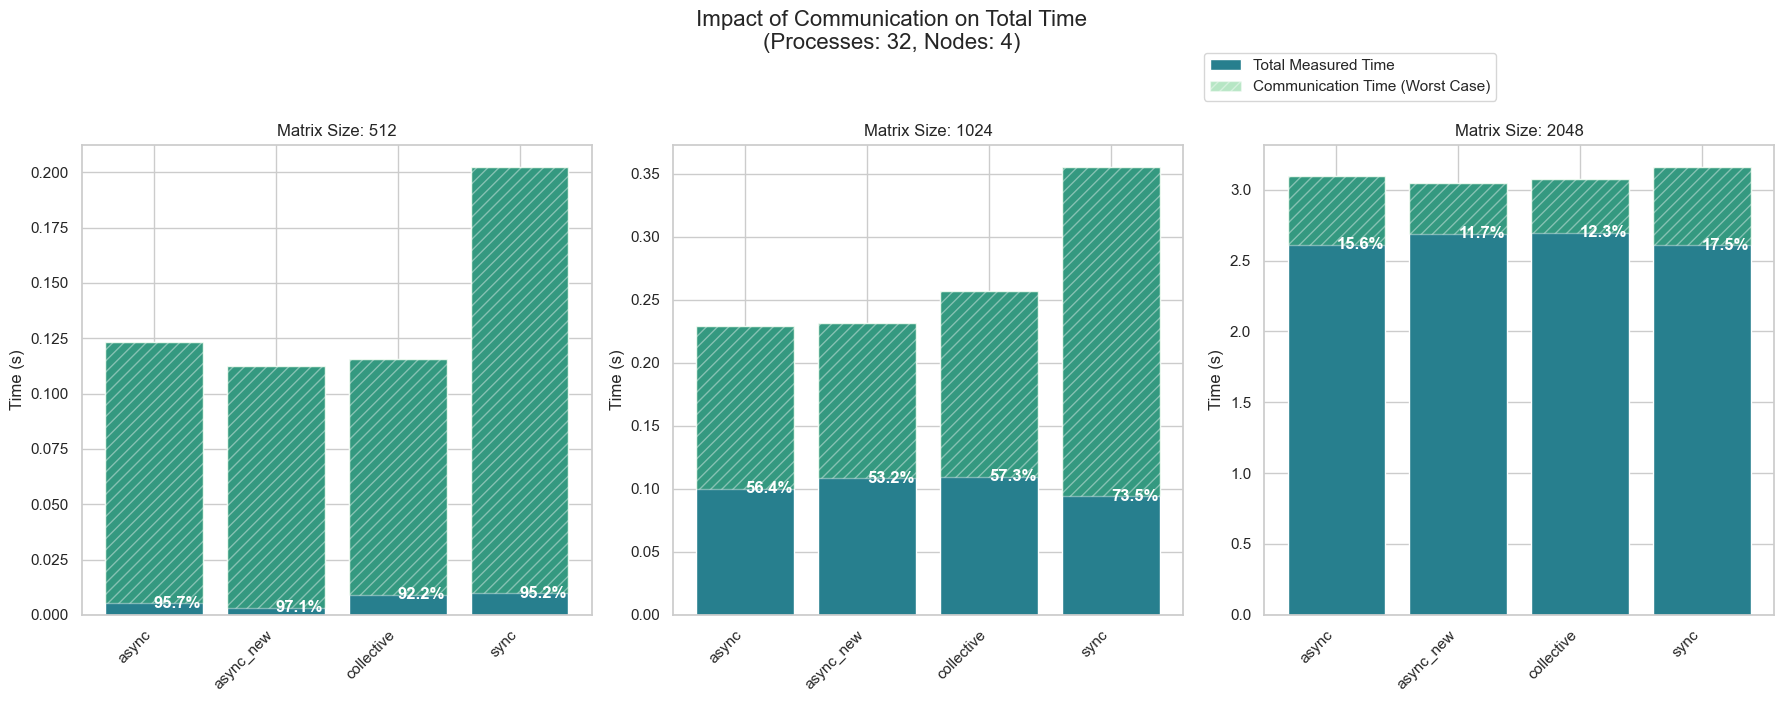
\includegraphics[width=1\linewidth]{images/comm_impact_4nodes.png}
    \caption{Impacto da comunicação no tempo total para 4 nós.}
    \label{fig:impact_4nodes}
\end{figure}

A observação dos gráficos resume bem nossa análise de desempenho:

1.  \textbf{O Custo da Comunicação Ineficiente:} Fica claro o problema da estratégia \texttt{sync} em múltiplos nós. Suas barras são as mais altas (pior desempenho) e a grande área listrada mostra que o culpado pelo mau desempenho é o tempo excessivo gasto na comunicação bloqueante.

2.  \textbf{O Benefício da Comunicação Eficiente:} Por outro lado, as estratégias \texttt{collective} e \texttt{async\_new} têm as barras mais curtas (melhor desempenho). Suas áreas de comunicação são bem menores, o que demonstra que otimizar a comunicação libera tempo para o que realmente importa: o cálculo.

3.  \textbf{Os Limites da Paralelização:} A matriz de 512x512 é um exemplo clássico dos limites da paralelização. O tempo total diminui de 1 para 2 nós, mas volta a aumentar com 3 e 4 nós. O motivo é claro: a área de comunicação se torna tão grande (acima de 90\%) que o custo de distribuir o trabalho supera qualquer ganho no cálculo. O problema é pequeno demais para ser distribuído eficientemente.

4.  \textbf{Paralelização Efetiva:} O comportamento da matriz de 2048x2048 é o oposto. O tempo total de execução cai drasticamente ao usar múltiplos nós, e a fração de tempo de comunicação se mantém baixa. Este é o cenário ideal, onde o problema é grande o suficiente para que a distribuição do trabalho compense o custo da comunicação em rede.

Em resumo, estes gráficos confirmam que a escolha de uma estratégia de comunicação eficiente é um fator determinante para o desempenho.

\subsection{Speedup de acordo com o numero de nodos}

A métrica final, e talvez a mais importante para avaliar o sucesso de uma aplicação paralela, é o \textit{speedup}. Ele mede o quanto ganhamos em desempenho ao adicionar mais recursos (neste caso, nós). O speedup é calculado como:
$$
\text{Speedup} = \frac{T_{\text{baseline}}}{T_{\text{paralelo}}}
$$
Aqui, nosso baseline é o tempo de execução em um único nó. Um speedup $> 1.0$ indica ganho de desempenho, enquanto um valor $< 1.0$ indica uma perda (slowdown).

As figuras \ref{fig:speedup_collective} a \ref{fig:speedup_async_new} apresentam o speedup para cada estratégia em formato de \textit{heatmap}, permitindo uma visualização rápida da escalabilidade.

\begin{figure}[H]
    \centering
    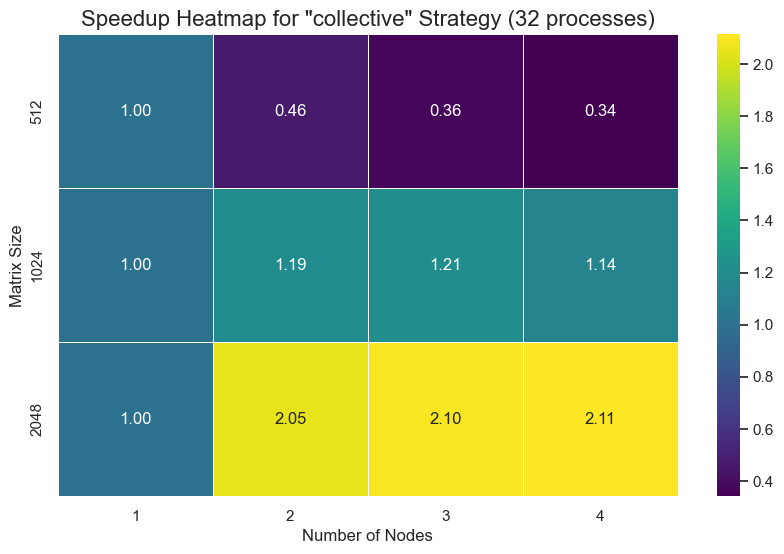
\includegraphics[width=0.8\linewidth]{images/speedup_collective.png}
    \caption{Heatmap do speedup de acordo com numero de nodos e tamanho da matriz para comunicação coletiva.}
    \label{fig:speedup_collective}
\end{figure}

\begin{figure}[H]
    \centering
    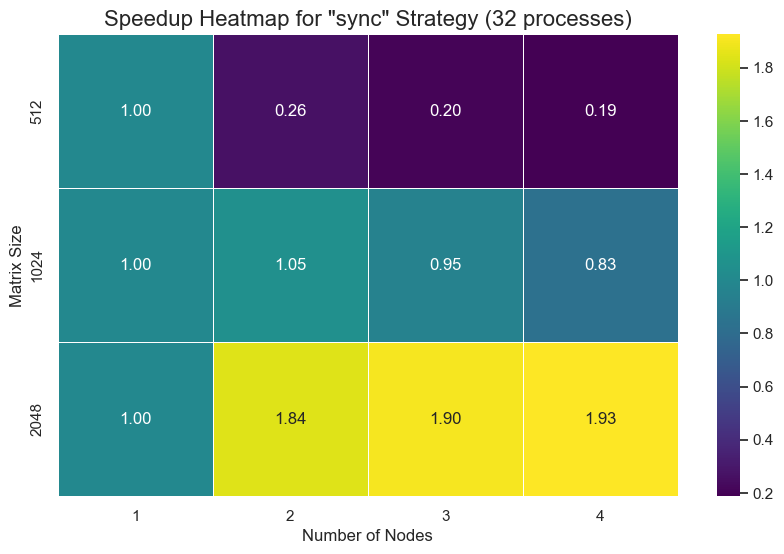
\includegraphics[width=0.8\linewidth]{images/speedup_sync.png}
    \caption{Heatmap do speedup de acordo com numero de nodos e tamanho da matriz para comunicação síncrona.}
    \label{fig:speedup_sync}
\end{figure}

\begin{figure}[H]
    \centering
    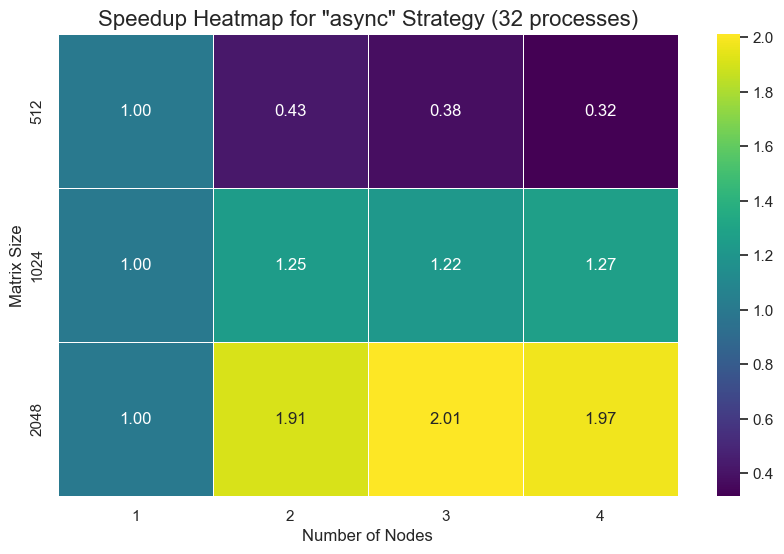
\includegraphics[width=0.8\linewidth]{images/speedup_async.png}
    \caption{Heatmap do speedup de acordo com numero de nodos e tamanho da matriz para comunicação assíncrona.}
    \label{fig:speedup_async}
\end{figure}

\begin{figure}[H]
    \centering
    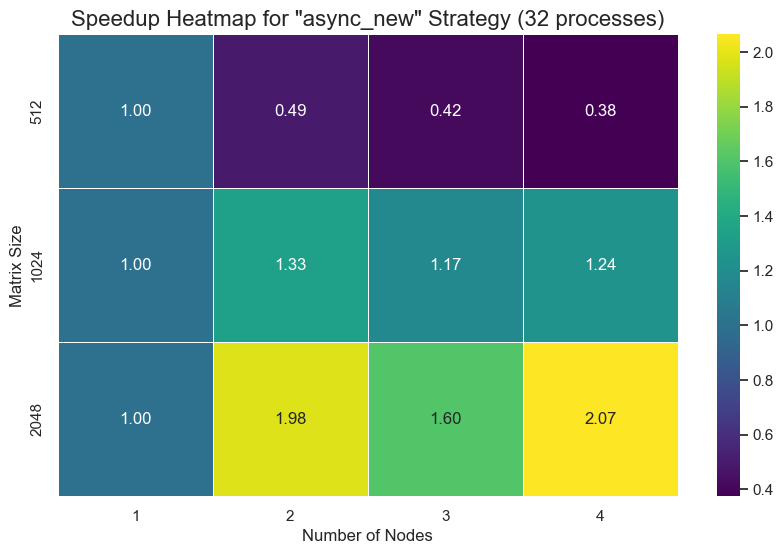
\includegraphics[width=0.8\linewidth]{images/speedup_async_new.png}
    \caption{Heatmap do speedup de acordo com numero de nodos e tamanho da matriz para comunicação assíncrona modificada.}
    \label{fig:speedup_async_new}
\end{figure}

A análise dos heatmaps deixa as conclusões bem claras:

1.  \textbf{O Tamanho do Problema é Essencial:} Para a matriz menor (512x512), \textbf{todas} as estratégias apresentaram slowdown (speedup $< 1.0$). Adicionar mais nós piorou o desempenho. Isso prova que, para problemas pequenos, o custo da comunicação em rede supera o benefício da paralelização.

2.  \textbf{A Ineficiência da Comunicação Síncrona:} O mapa de calor da estratégia \texttt{sync} (Figura \ref{fig:speedup_sync}) é o mais "frio", indicando o pior speedup. Mesmo para a maior matriz, o ganho foi baixo (1.93x). Essa abordagem simplesmente não escala bem.

3.  \textbf{Escalabilidade das Estratégias Eficientes:} As estratégias \texttt{collective} (Figura \ref{fig:speedup_collective}) e \texttt{async\_new} (Figura \ref{fig:speedup_async_new}) escalaram muito melhor. Para a matriz de 2048x2048, ambas alcançaram um speedup acima de 2.0x, mostrando que distribuem o trabalho de forma eficaz para problemas grandes.

4.  \textbf{Destaque para a \texttt{async\_new}:} A estratégia \texttt{async\_new} se destacou como a mais promissora, apresentando o melhor speedup na maioria dos cenários (atingindo 2.06x com 4 nós para a matriz de 2048x2048). O resultado anômalo (1.60x) com 3 nós para essa mesma matriz teve um desvio padrão muito alto nos dados brutos, sugerindo que essa medição específica pode ter sido afetada por algum fator externo. Desconsiderando essa anomalia, a tendência da \texttt{async\_new} é a de melhor escalabilidade.

Em suma, a análise de speedup consolida tudo o que vimos: para ter ganho de desempenho com mais hardware, é fundamental escolher uma estratégia de comunicação que minimize o tempo ocioso.

\section{Conclusão}
\

Este trabalho comparou o desempenho de estratégias de comunicação MPI (síncrona, assíncrona e coletiva) em um algoritmo de multiplicação de matrizes. Através de testes sistemáticos, conseguimos tirar conclusões claras sobre a eficiência e a escalabilidade de cada abordagem.

A análise mostrou que a escolha da estratégia de comunicação é um fator crítico para o desempenho, principalmente quando usamos múltiplos nós e a latência da rede entra em jogo. A comunicação síncrona (\texttt{sync}), embora simples, provou ser a mais ineficiente, causando perdas de desempenho (slowdown) na maioria dos cenários distribuídos por conta de sua natureza bloqueante.

Em contraste, as operações coletivas (\texttt{collective}) e nossa versão melhorada da não bloqueante (\texttt{async\_new}) foram as grandes vencedoras. A estratégia coletiva se mostrou robusta e rápida, alcançando um speedup de mais de 2.0x, o que confirma a alta otimização da biblioteca MPI. No entanto, a nossa implementação \texttt{async\_new} foi ainda mais promissora, apresentando o melhor desempenho e a maior escalabilidade na maioria dos testes.

O estudo também reforçou um princípio chave da computação paralela: a granularidade do problema. Para matrizes pequenas (512x512), o custo da comunicação foi maior que o ganho da paralelização. Apenas com matrizes grandes (2048x2048) o speedup foi significativo, pois o tempo economizado no cálculo compensou o custo da comunicação.

Concluímos, portanto, que para desenvolver aplicações MPI escaláveis, o uso de comunicação síncrona ponto-a-ponto deve ser evitado. A escolha entre operações coletivas e uma comunicação não bloqueante bem estruturada é o caminho para o alto desempenho. Este trabalho atingiu seus objetivos ao quantificar essas diferenças, confirmando que a otimização da comunicação é um pilar essencial da programação paralela e distribuída.


\end{document}